\section{MIMA}

\begin{frame}{MIMA}
    \centering
	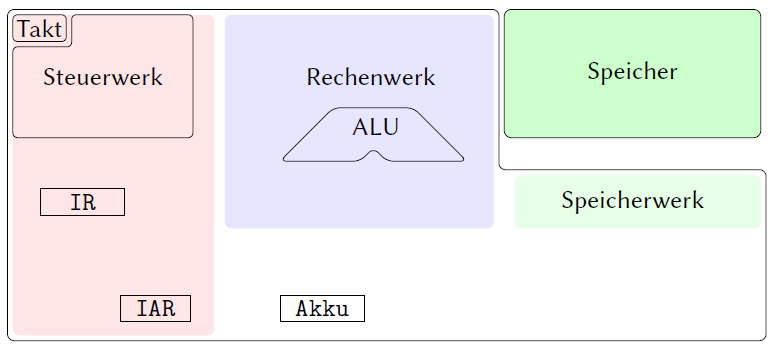
\includegraphics[width=.82\linewidth]{mima/MIMA_simple.png}\\
	Die \emph{MIMA} ist ein idealisierter Prozessor. 
\end{frame}

\begin{frame}{Eigenschaften}
	\begin{itemize}[<+->]
		\item Adressen sind 20 Bit lang
		\item \enquote{Werte} sind 24 Bit lang
		\item Befehlscodierungen -- zwei Formate:
		\begin{itemize}
			\item[a)] 4 Bit für den OpCode und 20 Bit für einen Parameter (Adresse / Konstante)
			\item[b)] 8 Bit Befehl (Rest irrelevant)\\
			\item[]<+(-2)-> \includegraphics[width=150px]{mima/MIMA_commands.png} 
		\end{itemize} 
	\end{itemize}
\end{frame}


\begin{frame}{Wichtige Register}
	\begin{itemize}[<+->]
		\item \emph{IAR} : InstruktionsAdressRegister : Speichert Adresse des aktuell auszuführenden Befehls.
		\item \emph{IR}: InstruktionsRegister : Speichert den auszuführenden Befehl selbst.
		\item \emph{SAR}: SpeicherAdressRegister : Enthält die Adresse eines Wertes, der aus dem Speicher gelesen werden soll.
		\item \emph{SDR}: SpeicherDatenRegister : Enthält einen Wert, der aus dem Speicher geladen wurde.
		\item \emph{Akku}: enthält Ausgangswerte/Ergebnisse von Berechnungen
	\end{itemize}
\end{frame}

\begin{frame}[t]{Aufbau}
	\begin{figure}
		\centering
		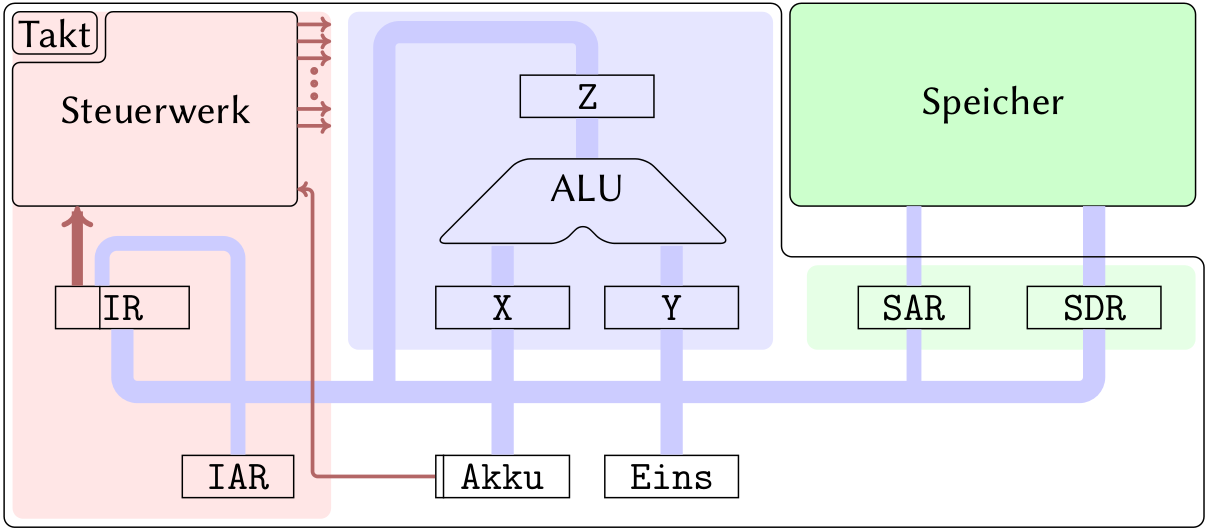
\includegraphics[width=.82\linewidth]{mima/MIMA.png}
	\end{figure}
\end{frame}

\begin{frame}[t]{Befehlsholphase}
	\begin{figure}
		\centering
		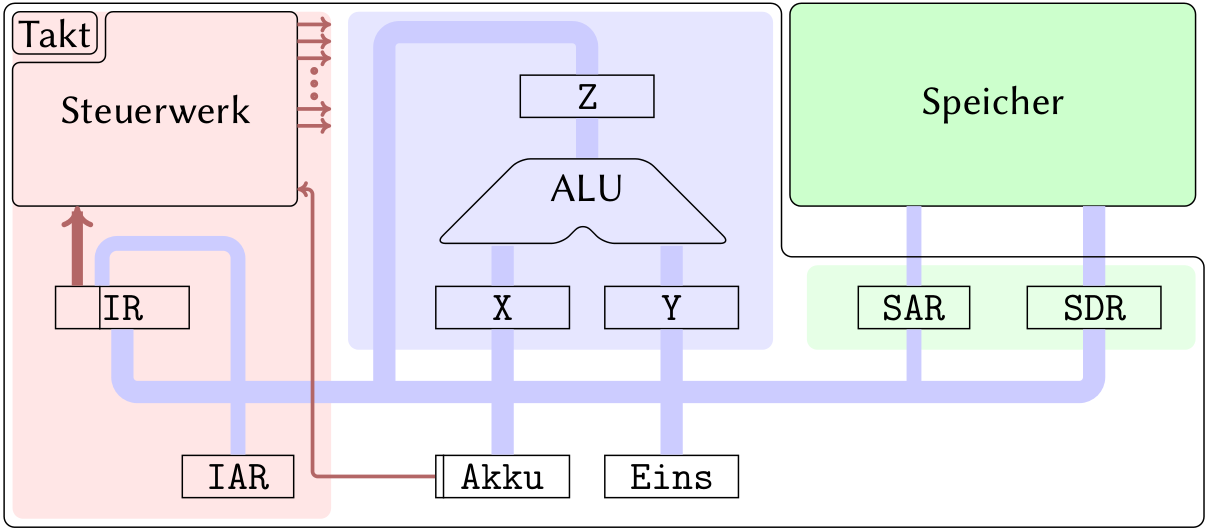
\includegraphics[width=.7\linewidth]{mima/MIMA.png}
	\end{figure}
	\pause
	\only<2-6>{\begin{itemize}
		\only<2|handout:1> {\item[1.] IAR $\to $ SAR  und IAR $\to$ X 
			\item[] Befehlsadresse dem Speicher übergeben und Zähler zum Erhöhen an ALU geben.}
		\only<3|handout:2>{\item[2.] Eins $\to$ Y  
			\item[] 1-Wert für Erhöhung des Zählers an ALU geben.}
		\only<4|handout:3>{\item[3.] ALU aufaddieren ($Z=X+Y$) 
			\item[] Nächste Befehlsadresse berechnen. }
		\only<5|handout:4>{\item[4.] Z $\to$ IAR 
			\item[] Adresse für nächste Runde speichern. }
		\only<6|handout:5>{\item[5.] SDR $\to$ IR 
			\item[] Wert zur angefragten Adresse erhalten. }
	\end{itemize}}	
\end{frame}

\newcommand{\itemizeconfig}{\setlength{\parsep}{0pt}\setlength{\parskip}{0pt}\setlength{\topsep}{0pt}\setlength{\partopsep}{0pt}}
\newcommand{\explain}[1]{\hfill {\small #1 }}
\begin{frame}{Befehle}
	Die MIMA besitzt einen Befehlssatz mit möglichen Befehlen. %Andere Befehle (oder Varianten) werden NICHT unterstützt und können daher nicht verwendet werden!
	\textbf{Nur die Befehle aus der VL} dürft ihr benutzen! \\ 
	\smallskip
	(Befehle, die eigentlich zwei Operanden brauchen, lesen zusätzl. vom Akku.)
	{
	\begin{itemize}[<+->] \itemizeconfig
		\item Rechenoperationen:
		\begin{itemize} 
			\item ADD adr \explain{Akku $\leftarrow$ Akku + mem(adr)}
			\item AND, OR, XOR adr \explain{Dasselbe mit bitweisem Und, Oder und eXclusive OR}
			\item NOT, RAR \explain{Akku $\leftarrow$ not(Akku); \quad  Rotate-Akku-Right();}
		\end{itemize}
		\item Datentransport:
		\begin{itemize}
			\item LDC const \explain{Akku $\leftarrow$ const\quad (const ist dabei eine \textbf{20-Bit}-Konstante) }
			\item LDV, STV adr \explain{(Lese/Schreibe in/vom Akku von/an Adresse)}
			\item LDIV, STIV adr \explain{(Lese/Schreibe von/an Adresse, die an der Adresse steht)}
		\end{itemize}
		\item Vergleichsoperation: EQL adr \explain{(liefert $-1$ wenn Akku $=$ mem(adr), 0 sonst)}
		\item Sprünge:
		\begin{itemize}
			\item JMP adr \explain{Springe zu Befehl in Adresse adr}
			\item JMN adr \explain{Springe, falls Akku negativ \quad „JuMp if Negative“}
		\end{itemize}
		\item HALT \explain{Stoppt die MIMA}
	\end{itemize}}
\end{frame}

\begin{frame}{Bemerkungen}
	\begin{block}{Indirekte Adressierung (LDIV, STIV)}
		\centering
		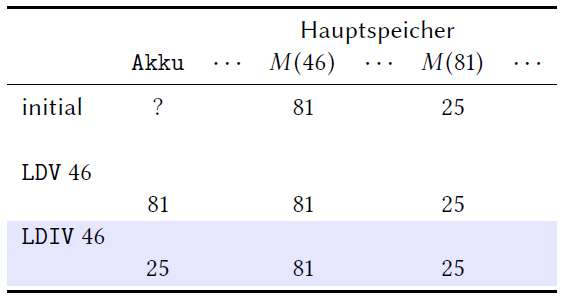
\includegraphics[width=250px]{mima/MIMA_indirect.png}
	\end{block}
	
\end{frame}

\begin{frame}{Bemerkungen}

	\begin{block}{HALT}
		Jedes Programm muss mit HALT enden! Sonst läuft das Programm endlos weiter! (Kostet dann Punkte!)
	\end{block}
	
    \pause
    
	\begin{block}{Negative Konstanten}
		Negative Konstanten können \textbf{nicht} mit LDC geladen werden. Warum? \\
		\pause \impl Unser Akku ist 24 Bit breit, aber wir können nur in die \textbf{hinteren 20 Bit} laden!
	\end{block}
\end{frame}

\begin{frame}{Negative Zahlen}
	\begin{block}{Aufgabe}
		An Adresse $a_1$ sei eine beliebige Zahl $x$ gegeben. Schreibt ein Programm, welches $-x$ (als Zweierkomplement) berechnet und an Adresse $a_2$ ablegt.
	\end{block}

	\visible<2|handout:2>{
		\begin{block}{Lösung}
			LDV $a_1$\\
			NOT\\
			STV $a_2$\\
			LDC 1\\
			ADD $a_2$\\
			STV $a_2$ \\
			HALT
		\end{block}
	}
\end{frame}

\begin{frame}{Beispiele}
	Beispiele zur Umsetzung von Anweisungen aus Hochsprachen (if, while, for....):\\
	\bigskip
	Siehe Übung Nr.~6 (WS 2018/19)
\end{frame}

\begin{frame}{Übung: Modulo 2 und Betrag}
	1. Schreibe ein Programm, das eine an Speicheradresse $a_1$ gegebenen positive Zahl Modulo 2 rechnet und an Adresse $a_2$ ablegt. \\
	\medskip
	2. Schreibe ein Programm, das den Betrag einer an Adresse $a_1$ gegebenen Zahl berechnet und an Adresse $a_2$ ablegt.
\end{frame}

\begin{frame}{Lösung: Modulo 2}
	\begin{tabbing}
		start: \; \= LDC 1 \quad  //$= 000000000000000000000001_2$ \\
				\> AND $a_1$ \\
				\> STV $a_2$ \\
				\> HALT
	\end{tabbing}
\end{frame}

\begin{frame}{Lösung: Betrag}
	\begin{tabbing}
		start: \quad \= LDV $a_1$ \\
					 \> JMN negate \\
		end: 		 \> STV $a_2$ \\
					 \> HALT \\
		negate:		 \> NOT \\
					 \> STV $a_2$ \\
					 \> LDC 1 \\
					 \> ADD $a_2$  \\
					 \> JMP end	 \\		 
	\end{tabbing}
\end{frame}

% \begin{frame}{Übung: Modulo 3}
% 	Schreibe ein Programm, das eine an Speicheradresse $a_1$ gegebenen positive Zahl Modulo \textbf{3} (drei!) rechnet und an Adresse $a_2$ ablegt.
% \end{frame}

% \begin{frame}{Lösung: Modulo 3}
%   \begin{tabbing}
%     start: \quad \= LDC 1 \\
%            \> STV One\\
%            \> LDC 3\\
%            \> NOT\\
%            \> ADD One\\
%            \> STV MinusThree\\
%            \> LDV $a_1$\\
%     \medskip
%     while: \> ADD MinusThree\\
%            \> JMN end\\
%            \> JMP while\\
%     \medskip
%     end:   \> STV $a_1$\\
%            \> LDC 3\\
%            \> ADD $a_1$\\
%            \> STV $a_2$ \\
%            \> HALT\\
%   \end{tabbing}
% \end{frame}